\documentclass{sajzk}

\usetikzlibrary {arrows.meta, angles, quotes}
\usetikzlibrary {calc}

\begin{document}
\section{Äußeres Produkt} 
\label{fuw3}
\lhead{:mathe:ga:}

Das äußere Produkt wurde von Hermann Grassmann eingeführt. Die moderne Variante des äußeren Produktes wird über die orientierte Fläche eines Parallelogramms definiert. Der Flächeninhalt wird als die Norm des Äußeren Produktes genannt.

$$
|u \wedge v| = |u| |v|\sin\alpha
$$

Zum Beispiel beschreiben die beiden äußeren Produkte $u\wedge v$ und
$\frac{1}{2}u\wedge 2v$ das selbe Objekt, wenn $u$ und $v$ Vektoren eines
n-Dimensionalen Raumes sind.

\begin{center}
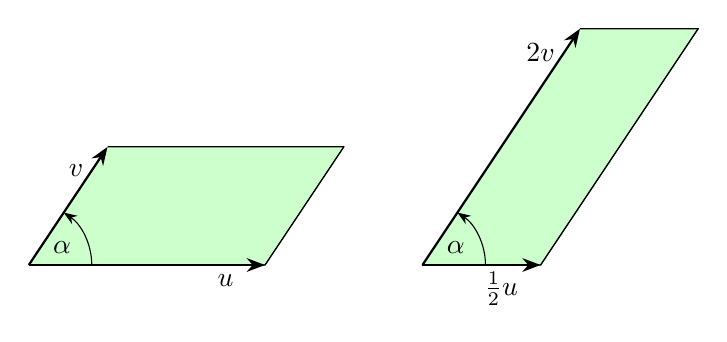
\begin{tikzpicture}[>=Stealth]
    \coordinate (A) at (0,0);
    \coordinate (B) at (3,0);
    \coordinate (C) at (4,1.5);
    \coordinate (D) at (1,1.5);

    \filldraw[fill=green!20] (A) -- (B) -- (C) -- (D);
    \draw[->, thick] (A) -- (B);
    \draw[->, thick] (A) -- (D);
    \draw (D) -- (C);
    \draw (B) -- (C);
    \node[shift={(-0.4,-0.3)}] (v) at (D) {$v$};
    \node[shift={(-0.5,-0.2)}] (u) at (B) {$u$};
    \pic ["$\alpha$", ->, draw=black, angle radius=0.8cm, angle eccentricity=0.6] {angle=B--A--D};

    \coordinate (A') at (5,0);
    \coordinate (B') at (6.5,0);
    \coordinate (C') at (8.5,3);
    \coordinate (D') at (7,3);

    \filldraw[fill=green!20] (A') -- (B') -- (C') -- (D');
    \draw[->, thick] (A') -- (B');
    \draw[->, thick] (A') -- (D');
    \draw (D') -- (C');
    \draw (B') -- (C');
    \node[shift={(-0.5,-0.3)}] (v) at (D') {$2v$};
    \node[shift={(-0.5,-0.3)}] (u) at (B') {$\frac{1}{2}u$};
    \pic ["$\alpha$", ->, draw=black, angle radius=0.8cm, angle eccentricity=0.6]
    {angle=B'--A'--D'};
\end{tikzpicture}
\end{center}

Die Orientierung der Fläche wird über die Reihenfolge der Vektoren in dem
Produkt erklärt.
\newpage
\subsection{Referenzen} 
\begin{itemize}
    \item \href{16ea.pdf}{Grassmanns Idee} 16ea.tex
    \item \href{f35d.pdf}{Geometrische Algebra} f35d.tex
    \item \href{81js.pdf}{Geometrisches Produkt} 81js.tex
    \item \href{vc8d.pdf}{Eingenschaften des äußeren Produkts} vc8d.tex
\end{itemize}

\subsection{Literatur} 
\begin{itemize}
    \item Alan Macdonald - Linear and Geometric Algebra (2021) Seite 76
    \item Hermann Grassmann - Projektive Geometrie der Ebene Unter Benutzung der Punktrechnung Dargestellt Erster Band Binäres (1909)
\end{itemize}
\end{document}
